\documentclass[tikz,border=8pt]{standalone}
% Shared look for every TikZ diagram. Load with \input{../../tools/tikz-style.tex}
\usepackage[T1]{fontenc}
\usepackage{lmodern}
\renewcommand{\sfdefault}{lmr}  % diagrams use the same serif as the text
\usetikzlibrary{arrows.meta, positioning, shapes.geometric, calc, fit, backgrounds}
\definecolor{cblue}{HTML}{4C78A8}
\definecolor{corange}{HTML}{F58518}
\definecolor{cgreen}{HTML}{54A24B}
\definecolor{cred}{HTML}{E45756}
\definecolor{cpurple}{HTML}{B279A2}
\definecolor{cgrey}{HTML}{6B6B6B}
\tikzset{
  every picture/.style={font=\sffamily, line width=1.2pt},
  box/.style={draw=#1, fill=#1!12, rounded corners=4pt, align=center, inner sep=7pt, minimum height=1.1cm},
  box/.default=cgrey,
  arrow/.style={-{Stealth[length=3mm]}, draw=cgrey, line width=1.4pt},
  title/.style={font=\sffamily\bfseries\Large},
  note/.style={font=\sffamily\small, text=cgrey, align=center},
}
\AtBeginDocument{\hyphenpenalty=10000 \exhyphenpenalty=10000}

\begin{document}
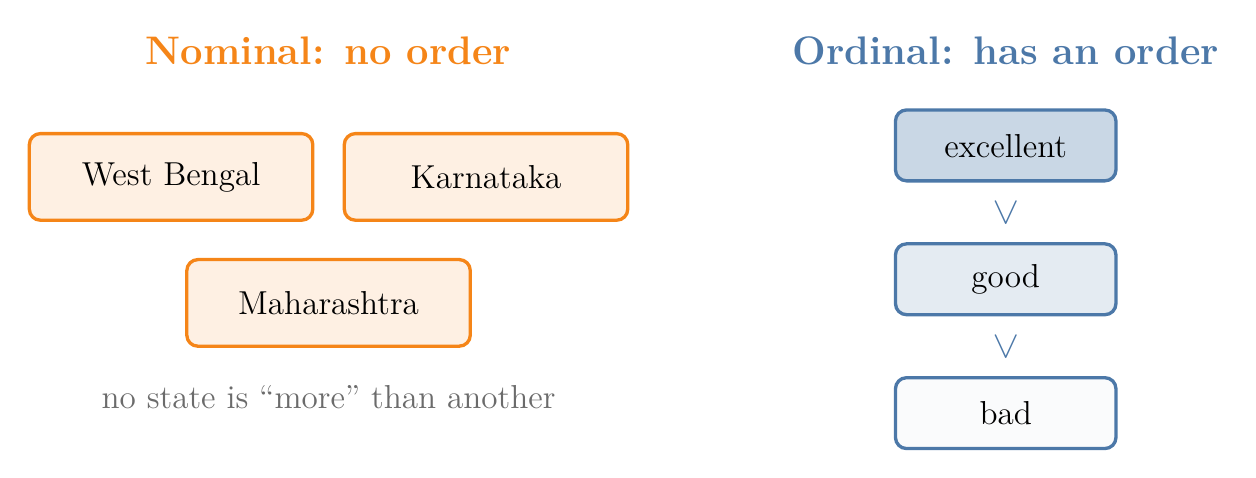
\begin{tikzpicture}[every node/.append style={font=\sffamily\large}]
\tikzset{note/.style={font=\sffamily\large, text=cgrey, align=center}}
  \node[title, text=corange] at (2.6,1.6) {Nominal: no order};
  \foreach \t/\x in {West Bengal/0, Karnataka/0, Maharashtra/0} {}
  \node[box=corange, minimum width=3.6cm] at (0.6,0) {West Bengal};
  \node[box=corange, minimum width=3.6cm] at (4.6,0) {Karnataka};
  \node[box=corange, minimum width=3.6cm] at (2.6,-1.6) {Maharashtra};
  \node[note] at (2.6,-2.8) {no state is ``more'' than another};
  \begin{scope}[xshift=9.6cm]
  \node[title, text=cblue] at (1.6,1.6) {Ordinal: has an order};
  \node[box=cblue, minimum width=2.8cm, minimum height=0.9cm, fill=cblue!30] (e) at (1.6,0.4) {excellent};
  \node[box=cblue, minimum width=2.8cm, minimum height=0.9cm, fill=cblue!15] (g) at (1.6,-1.3) {good};
  \node[box=cblue, minimum width=2.8cm, minimum height=0.9cm, fill=cblue!3] (b) at (1.6,-3.0) {bad};
  \node[font=\Large, text=cblue] at (1.6,-0.45) {\rotatebox{-90}{$>$}};
  \node[font=\Large, text=cblue] at (1.6,-2.15) {\rotatebox{-90}{$>$}};
  \end{scope}
\end{tikzpicture}
\end{document}
